% !TEX root = ../main.tex
\lecture{2}{2026-09-21}{Woche 2}

\textbf{Vorlesungsfolien} \url{https://moodle-app2.let.ethz.ch/course/section.php?id=261070}

\subsection{Vektoren}
\textbf{Definition} \textit{Vektoren} sind Elemente aus n-Dimensionalen Mengen.
\begin{theorem}
    $\textbf{x}$ oder $ \vec{x} = $
    $\begin{pmatrix}
        x_1 \\
        \vdots\\ 
        x_n
    \end{pmatrix}$
    $\in \mathbb{R}^n$
\end{theorem}

\subsubsection{Skalare Multiplikation}

Eindimensionale Zahl multipliziert Vektor 

\begin{theorem}
    \textbf{$\alpha$x} oder  $\vec{\alpha x} = $
    $\begin{pmatrix}
       \alpha x_1 \\
        \vdots\\ 
       \alpha x_n
    \end{pmatrix}$
    $\in \mathbb{R}^n$
\end{theorem}

Laenge oder \textit{euklidische}\textbf{Norm} von $x \in \mathbb{R}^n ist$
\pagebreak

\subsubsection{$\epsilon$-Umgebung}

\begin{theorem}
    Sei \textbf{x}  $\in \mathbb{R}^n$, $\epsilon \in \mathbb{R}, \epsilon > 0$ Dann ist 
    \begin{equation}
        U(\textbf{x}, \epsilon) = \left\{\textbf{y} \in \mathbb{R}^n \middle| \lVert\textbf{y}-\textbf{x}\rVert = \sqrt{\sum_{i=1}^{n} (y_i - x_i)^2} < \epsilon\right\}
   \end{equation}   
   Beschreibt alle Abstandsvektoren mit maximaler Länge $\epsilon$ von $X$. 
\end{theorem}

\textbf{$\epsilon$-Umgebungen sind immer konvex.}

\begin{center}
    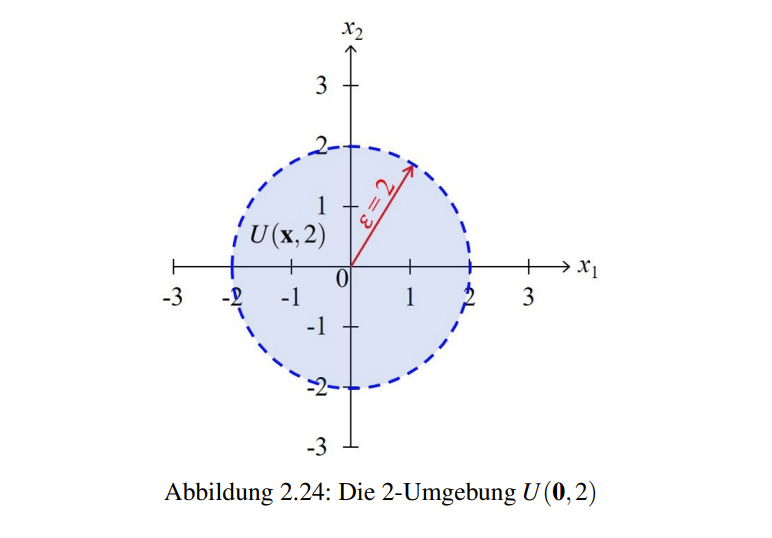
\includegraphics[width=\linewidth]{figures/epsilon_umgebung.png}
\end{center}

\subsection{Konvexe Mengen}
\begin{definition}
    [Konvexe Menge] Wenn jeder Punkt einer Verbindungslinie zwischen zwei Punkte einer Menge auch in zur Menge gehören, ist sie dann konvex.
    
\end{definition}

\subsubsection{Konvexe Kombination}
Punkte auf Verbindungslinie von Y und X mit $ 0 \le \alpha \le 1$ beschrieben. Sonst fuer $\alpha$ ausserhalb dieser schranke besteht eine allgemeine Gerade

\begin{theorem}
    Für $\vec{x}, \vec{y} \in \mathbb{R}^n$ und $0 \le \alpha \le 1$ beschreibt der resultierende Vektor die Differenz [Abstand] von $\vec{y}$ zu $\vec{x}$ in Abhängigkeit von $\alpha$.
    \begin{equation}
        \label{eq:kon_komb}
        a = \alpha \vec{x} + (1-\alpha) \vec{y} = \vec{y} + \alpha (\textbf{x} - \textbf{y}) = \vec{y} + \alpha (\vec{yx})
    \end{equation}

    Bei $\alpha = 0$ ist $ \vec{a} = \vec{y} $ und $\alpha = 1 \implies \vec{a} = \vec{x}$
\end{theorem}

\begin{definition} [Konvexe Menge]
    Formell gilt für eine konvexe Menge.
        \begin{equation}
        a = \alpha \vec{x} + (1-\alpha) \vec{y} = \vec{y} + \alpha (\textbf{x} - \textbf{y}) = \vec{y} + \alpha (\vec{yx}) \in \mathbb{A}
    \end{equation}
    Also wenn jeder beliebigen Punkt zwischen Y und X (beschrieben durch $\alpha$) auch in der Menge liegt.
\end{definition}

\begin{theorem}
    Der Durchschnitt $P = H_1 \cap H_2 \cap \dots \cap H_n$ konvexer Mengen ist immer Konvex
\end{theorem}

\begin{theorem}
    Das Komplement $P = H_1 \setminus H_2 \setminus \dots \setminus H_n$ ist \textbf{nicht} immer konvex.
\end{theorem}


\subsubsection{Innere, Aeusere, Randpunkte}

\textbf{Definition} fuer einen Innerenpunkt existiert immer eine $\epsilon$-Umgebung 

\subsubsection{Offene und abgeschlossene Mengen}

Offen gilt wenn eine Menge so definiert ist, dass seine Randpunkte die Definition nicht erfuellen A = (1,4) beschreibt alles zwischen 1 und 4 ohne sie selber, also offen.
Gleich bei $\epsilon$-Umgebungen, worin die Laenge \textbf{kleiner} als $\epsilon$ sind. 

Allgemein Abgeschlossene, nicht offene mengen, ist mindestens ein Randpunkt in der Menge drin. Unten beschraenkt, gibt Objekt der kleiner ist als alle Objekten der Mengen. Oben beschraenkt, es gibt Element ausserhalb der Menge, der groesser ist als alle in der Menge. 
Wenn oben und unten beschraenkt dann ist die Menge \textbf{kompakt}

\subsection{Supremum, Infimum, Maximum, Minimum}

\begin{definition}
   [Infimum] Ist $ A \subseteq \mathbb{R}$ nach unten beschraenkt, heisst die grösste untere Schranke \textit{inf}A. Oder Element zu dem alle anderen grösser oder gleich sind.
\end{definition}

\begin{definition}
    [Minimum] wenn eine Menge ihr \textit{Infimum} beinhaltet, ist es ihr \textit{min}.
    \begin{equation}
         infA \subseteq A \implies minA = infA
    \end{equation}
\end{definition}

\begin{definition}
    [Supremum und Maximum] gleiche Logik für obere Schranke und grösstes Element.
\end{definition}